\documentclass[11pt]{article}
\usepackage{geometry,marginnote} % Pour passer au format A4
\geometry{hmargin=1cm, vmargin=1cm} % 

% Page et encodage
\usepackage[T1]{fontenc} % Use 8-bit encoding that has 256 glyphs
\usepackage[english,french]{babel} % Français et anglais
\usepackage[utf8]{inputenc} 

\usepackage{lmodern,numprint}
\setlength\parindent{0pt}

% Graphiques
\usepackage{graphicx,float,grffile,units}
\usepackage{tikz,pst-eucl,pst-plot,pstricks,pst-node,pstricks-add,pst-fun,pgfplots} 

% Maths et divers
\usepackage{amsmath,amsfonts,amssymb,amsthm,verbatim}
\usepackage{multicol,enumitem,url,eurosym,gensymb,tabularx}

\DeclareUnicodeCharacter{20AC}{\euro}



% Sections
\usepackage{sectsty} % Allows customizing section commands
\allsectionsfont{\centering \normalfont\scshape}

% Tête et pied de page
\usepackage{fancyhdr} \pagestyle{fancyplain} \fancyhead{} \fancyfoot{}

\renewcommand{\headrulewidth}{0pt} % Remove header underlines
\renewcommand{\footrulewidth}{0pt} % Remove footer underlines

\newcommand{\horrule}[1]{\rule{\linewidth}{#1}} % Create horizontal rule command with 1 argument of height

\newcommand{\Pointilles}[1][3]{%
  \multido{}{#1}{\makebox[\linewidth]{\dotfill}\\[\parskip]
}}

\newtheorem{Definition}{Définition}

\usepackage{siunitx}
\sisetup{
    detect-all,
    output-decimal-marker={,},
    group-minimum-digits = 3,
    group-separator={~},
    number-unit-separator={~},
    inter-unit-product={~}
}

\setlength{\columnseprule}{1pt}

\begin{document}

\textbf{Nom, Prénom :} \hspace{8cm} \textbf{Classe :} \hspace{3cm} \textbf{Date :}\\

\begin{center}
  \textit{Si nous faisions tout ce dont nous sommes capables, nous nous surprendrions vraiment.}  - \textbf{Thomas Edison}
\end{center}

\subsubsection*{Cours}
\textbf{Théorème de Pythagore : } \dotfill \\
\Pointilles[1]

\subsubsection*{Pythagore rapide}
\textbf{Écrire le calcul et le résultat.}
  
\begin{figure}[H]
  \centering
  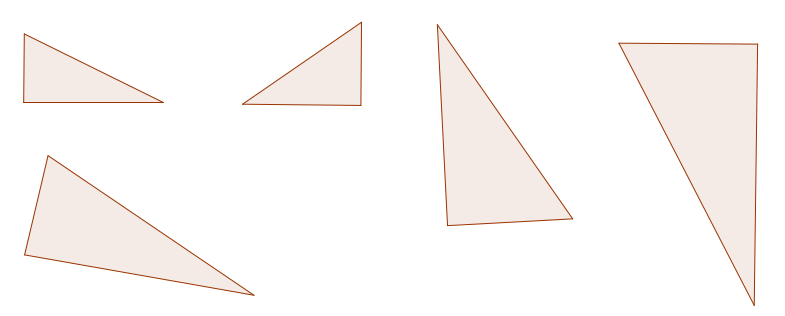
\includegraphics[width=0.8\linewidth]{4x6-Pythagore/ex2.png}
\end{figure}

\begin{multicols}{5}
  \begin{enumerate}
  \item[a.] \dotfill 
  \item[b.] \dotfill
  \item[c.] \dotfill 
  \item[d.] \dotfill 
  \item[e.] \dotfill 
  \end{enumerate}
\end{multicols}
\Pointilles[1]

\subsubsection*{Pythagore rédigé}

\begin{multicols}{3}
\begin{enumerate}
  \item[a.]Soit PVR un triangle rectangle en V tel que : RV = 17,5 cm et RP = 18,5 cm. \\
  \textbf{Calculer la longueur PV.}

  \item[b.]Soit LQF un triangle rectangle en F tel que : QF = 4,8 m et LF = 2 m. \\
  \textbf{Calculer la longueur QL.}

  \item[c.]Soit JMR un triangle rectangle en R tel que : MJ = 2,9 cm et MR = 2,1 cm. \\
  \textbf{Calculer la longueur JR.}
\end{enumerate}
\end{multicols}

\Pointilles[14]
\newpage

\subsubsection*{Pythagore problèmes}

\begin{multicols}{2}
\begin{enumerate}
  \item[pb1.] Pour être en sécurité une échelle de 5m doit être écarté de 1,5m du mur.\\
    \textbf{Quelle hauteur maximal peut-on atteindre ?}

  \item[pb2.] Afin de faire un avion, on plie une feuille A4 de dimension $21cm \times 29,7cm$ selon la figure ci-contre.\\
    \textbf{Calculer le périmètre et l'aire de la figure.}

  \begin{figure}[H]
    \centering
    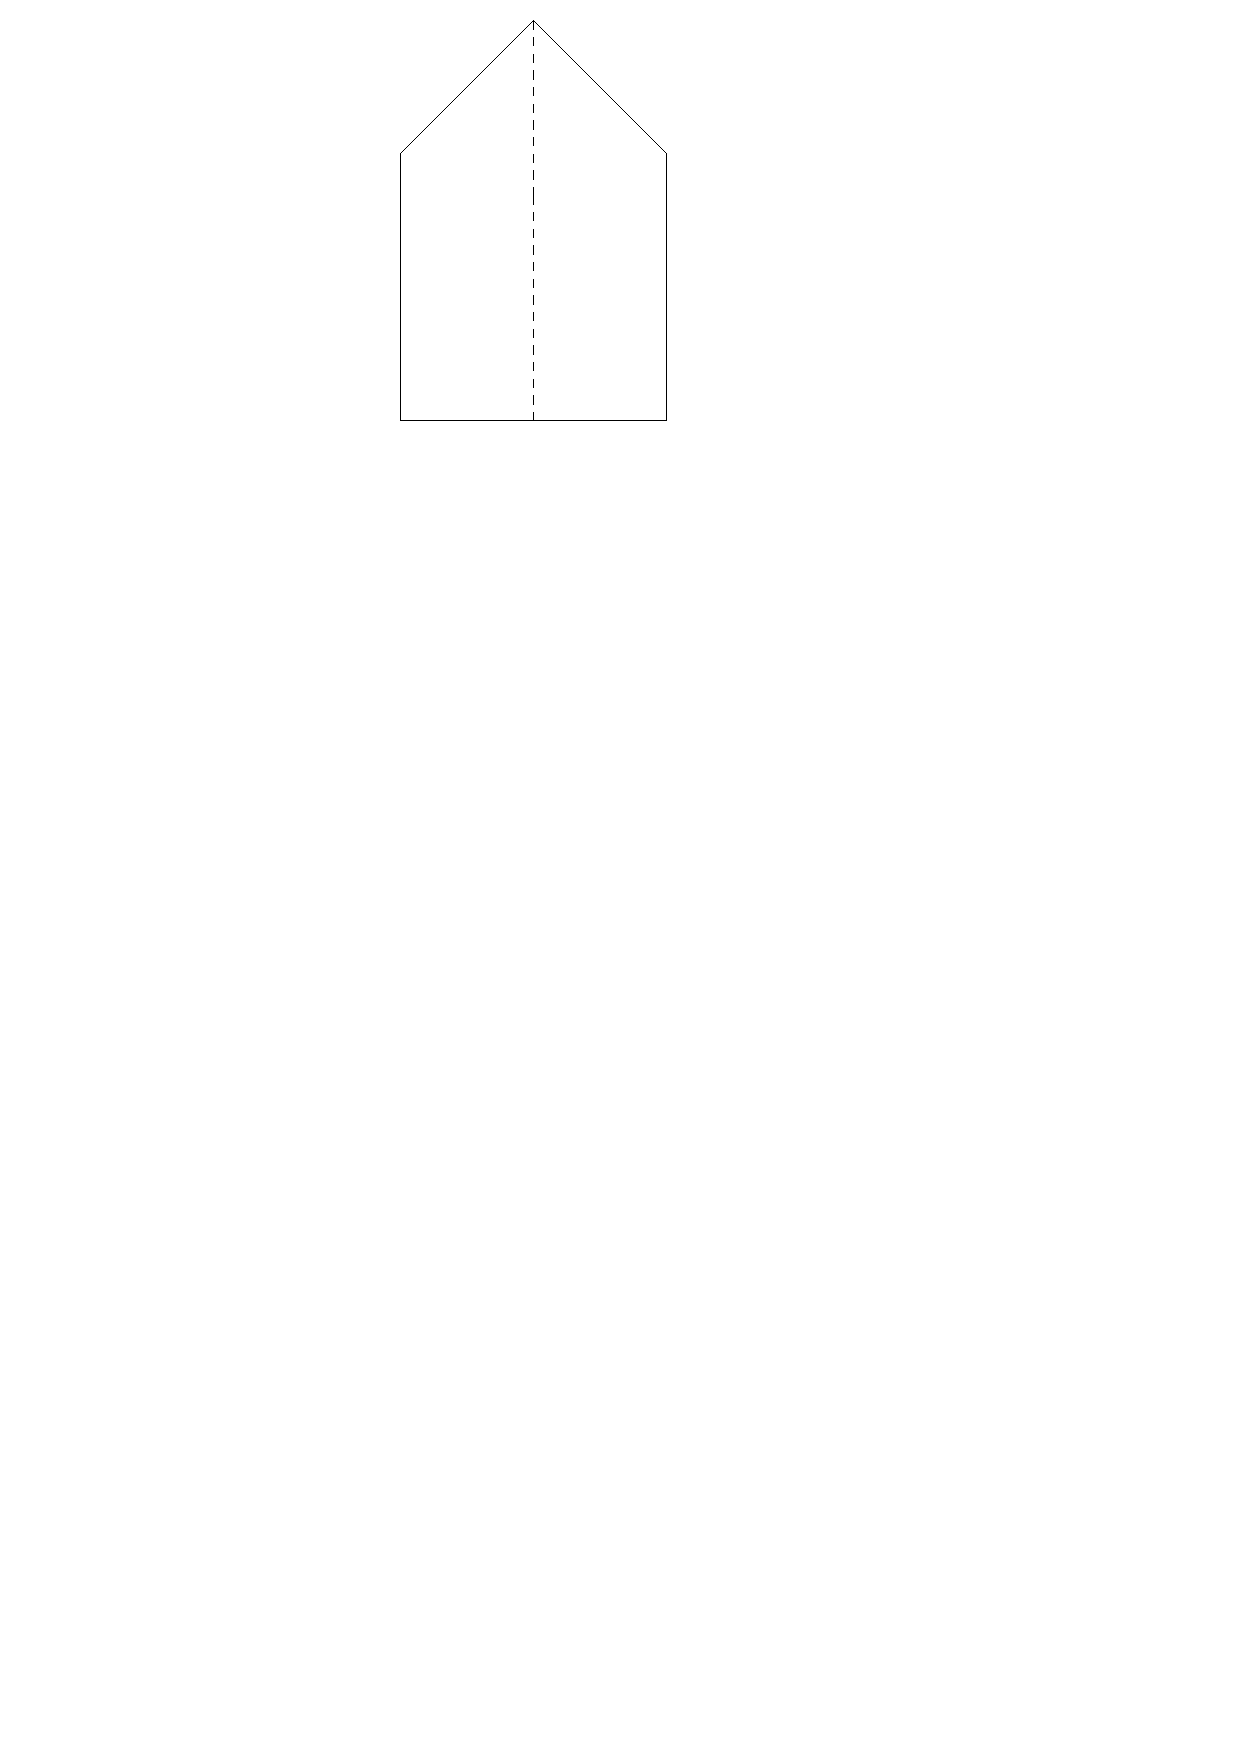
\includegraphics[width=0.4\linewidth]{4x6-Pythagore/pb2.pdf}
  \end{figure}
\end{enumerate}
\end{multicols}

\begin{multicols}{2}
  \begin{enumerate}
  \item[pb3.] \textit{À Pise vers 1200 après J. C. (problème attribué à Léonard de Pise, dit Fibonacci, mathématicien italien   du moyen âge).} \\
  Une lance de 6m est posée verticalement le long d’une tour considérée comme perpendiculaire au sol. \\
  Si on éloigne l’extrémité de la lance qui repose sur le sol de 3,6m de la tour, de  \textbf{combien descend l’autre extrémité de la lance le long du mur ?}

  \begin{figure}[H]
    \centering
    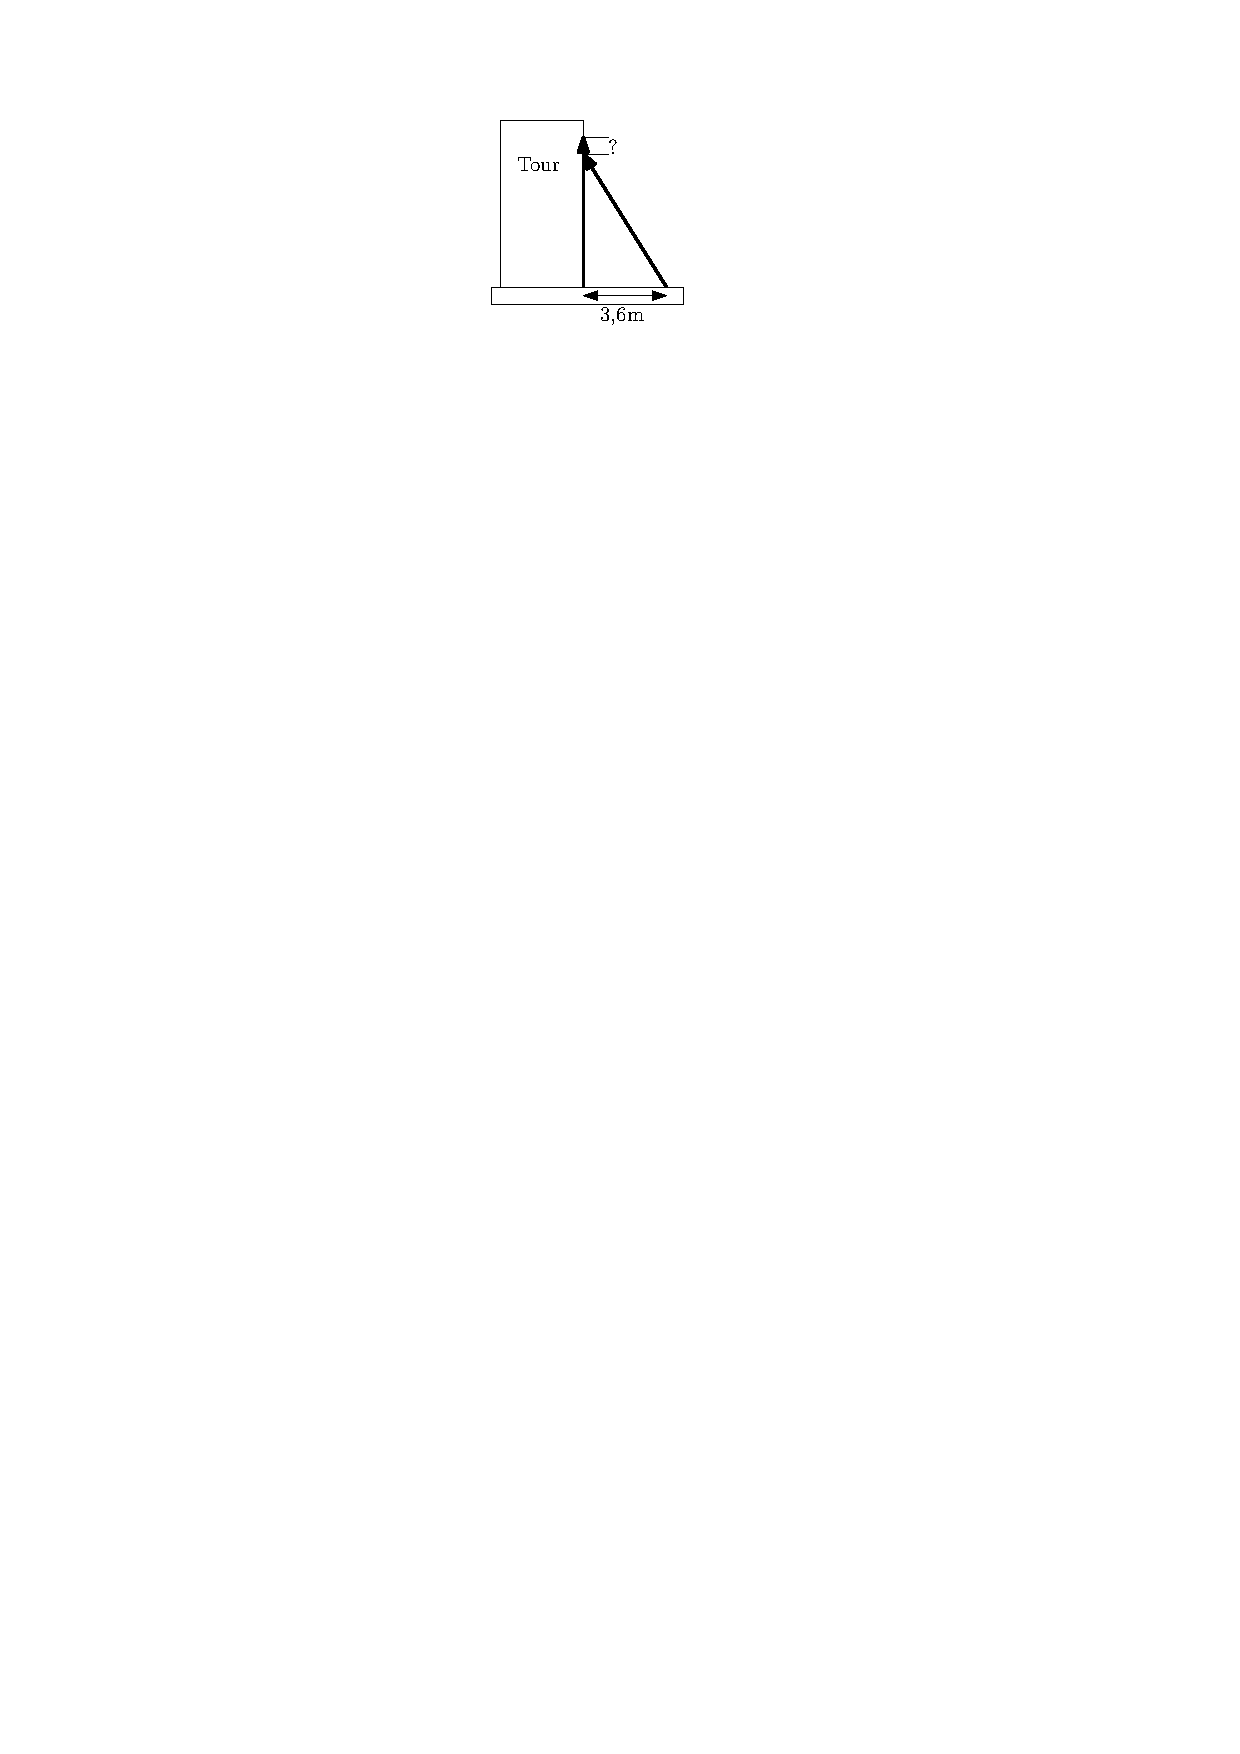
\includegraphics[width=0.6\linewidth]{4x6-Pythagore/pb3.pdf}
  \end{figure}
\end{enumerate}
\end{multicols}

\begin{enumerate}
  \item[pb4.] Fatma doit consolider et réparer un pont qui a été endommagé et qui risque de s'effondrer. Elle doit fixer 12 renforts en bois sur les poteaux verticaux qui soutiennent le ponton, comme le montre le dessin. \\
    \textbf{Calculer la longueur d'un renfort puis calculer la longueur totale de tous les renforts nécessaires}. 
  
    \begin{figure}[H]
    \centering
    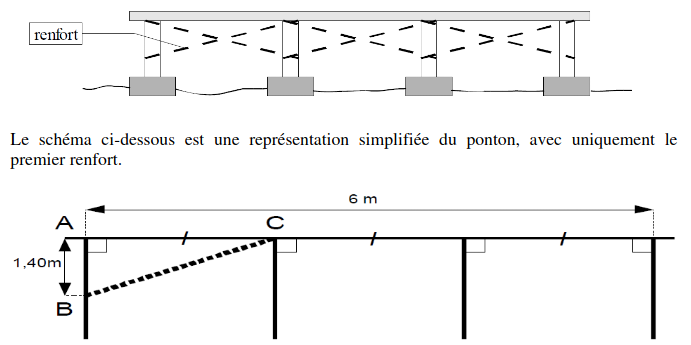
\includegraphics[width=0.8\linewidth]{4x6-Pythagore/pb4.png}
  \end{figure}
\end{enumerate}

\newpage


\textbf{Nom, Prénom :} \hspace{8cm} \textbf{Classe :} \hspace{3cm} \textbf{Date :}\\

\begin{center}
  \textit{Si nous faisions tout ce dont nous sommes capables, nous nous surprendrions vraiment.}  - \textbf{Thomas Edison}
\end{center}

\subsubsection*{Cours}
\textbf{Théorème de Pythagore : } \dotfill \\
\Pointilles[1]

\subsubsection*{Pythagore rapide}
\textbf{Écrire le calcul et le résultat.}
  
\begin{figure}[H]
  \centering
  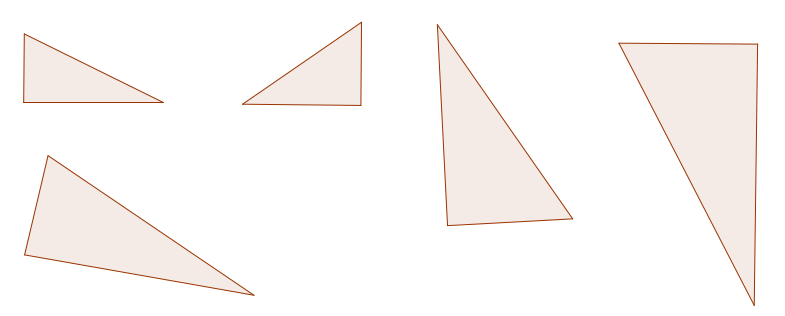
\includegraphics[width=0.8\linewidth]{4x6-Pythagore/ex2.png}
\end{figure}

\begin{multicols}{5}
  \begin{enumerate}
  \item[a.] \dotfill 
  \item[b.] \dotfill
  \item[c.] \dotfill 
  \item[d.] \dotfill 
  \item[e.] \dotfill 
  \end{enumerate}
\end{multicols}
\Pointilles[1]

\subsubsection*{Pythagore rédigé}

\begin{multicols}{3}
\begin{enumerate}
  \item[a.]Soit PVR un triangle rectangle en P tel que : RV = 27,5 cm et RP = 18,5 cm. \\
  \textbf{Calculer la longueur PV.}

  \item[b.]Soit LQF un triangle rectangle en L tel que : QF = 4,8 m et LF = 2 m. \\
  \textbf{Calculer la longueur QL.}

  \item[c.]Soit JMR un triangle rectangle en M tel que : MJ = 2,9 cm et MR = 2,1 cm. \\
  \textbf{Calculer la longueur JR.}
\end{enumerate}
\end{multicols}

\Pointilles[14]
\newpage

\subsubsection*{Pythagore problèmes}

\begin{multicols}{2}
\begin{enumerate}
  \item[pb1.] Pour être en sécurité une échelle de 5m doit être écarté de 1,5m du mur.\\
    \textbf{Quelle hauteur maximal peut-on atteindre ?}

  \item[pb2.] Afin de faire un avion, on plie une feuille A4 de dimension $21cm \times 29,7cm$ selon la figure ci-contre.\\
    \textbf{Calculer le périmètre et l'aire de la figure.}

  \begin{figure}[H]
    \centering
    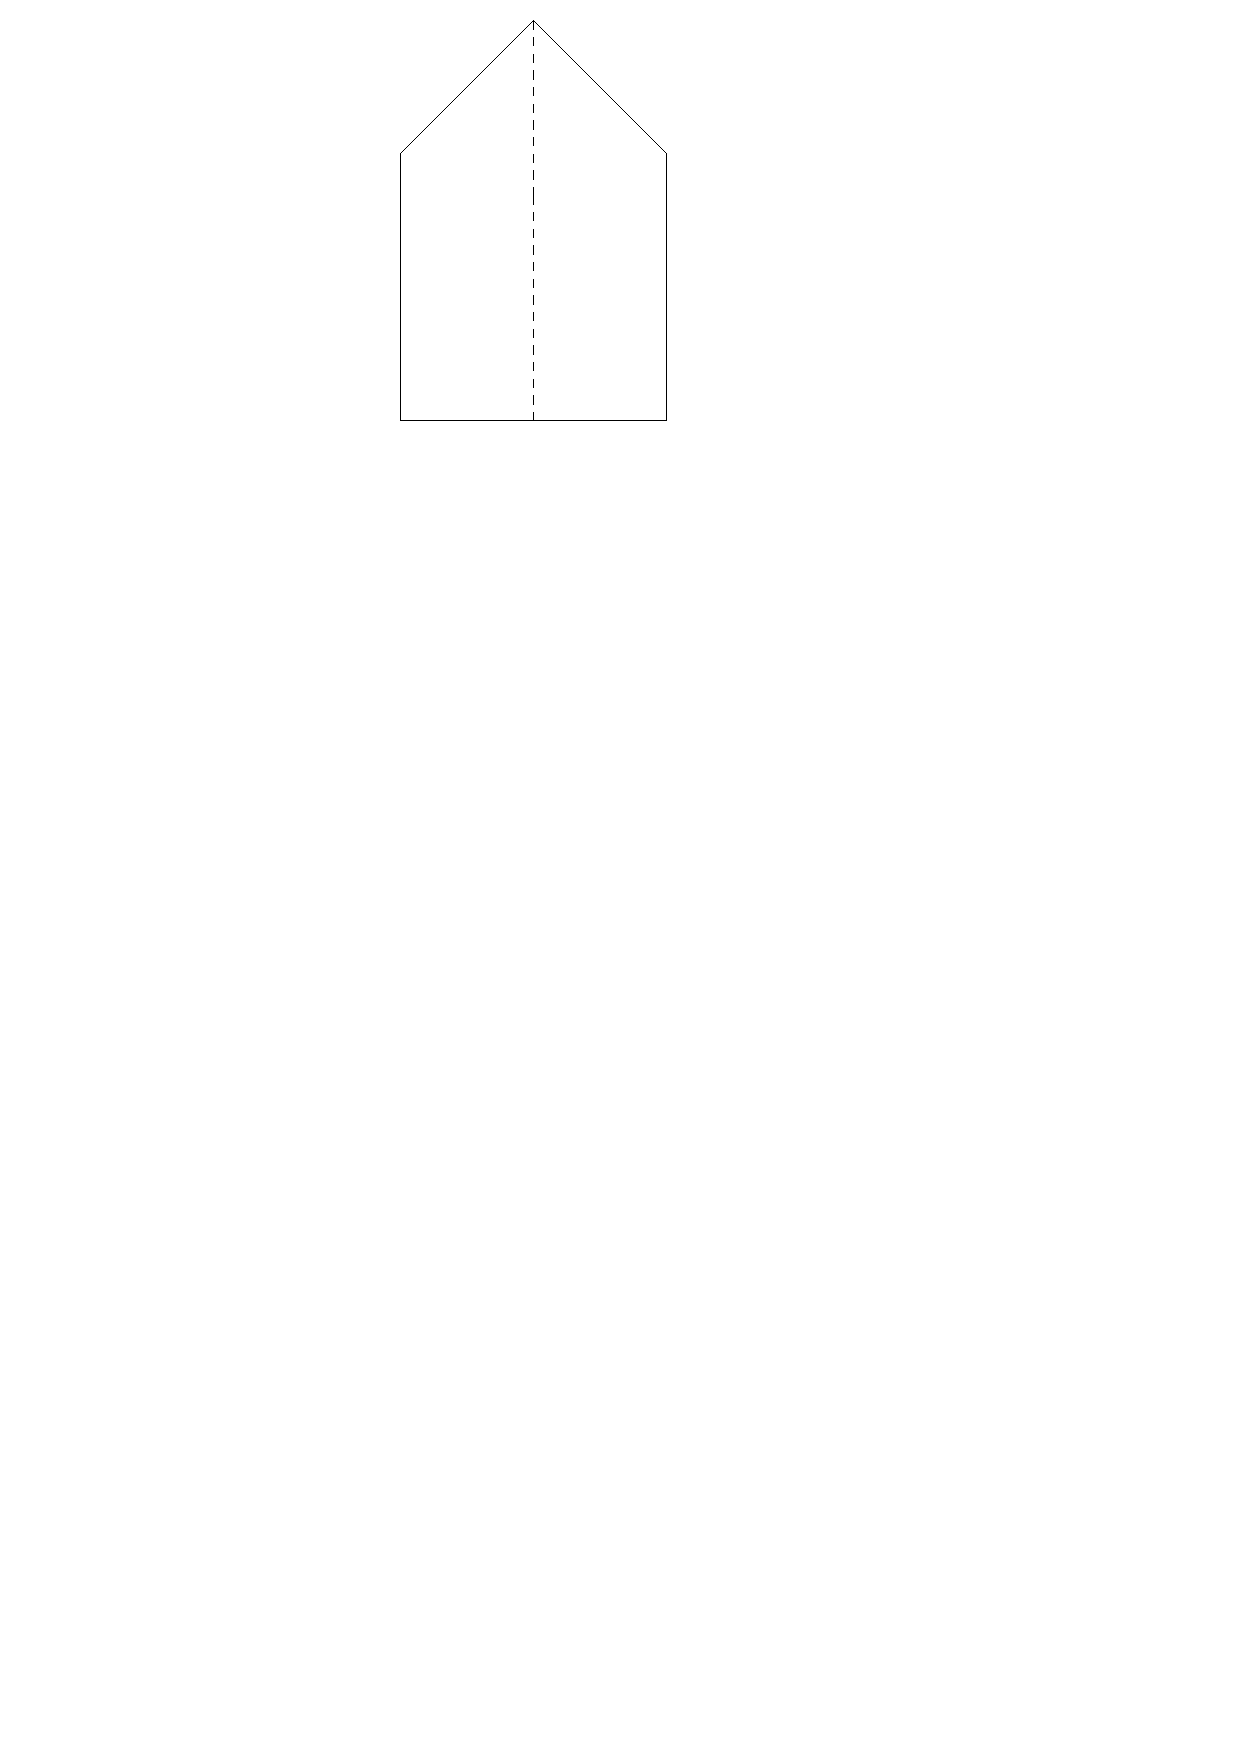
\includegraphics[width=0.4\linewidth]{4x6-Pythagore/pb2.pdf}
  \end{figure}
\end{enumerate}
\end{multicols}

\begin{multicols}{2}
  \begin{enumerate}
  \item[pb3.] \textit{À Pise vers 1200 après J. C. (problème attribué à Léonard de Pise, dit Fibonacci, mathématicien italien   du moyen âge).} \\
  Une lance de 6m est posée verticalement le long d’une tour considérée comme perpendiculaire au sol. \\
  Si on éloigne l’extrémité de la lance qui repose sur le sol de 3,6m de la tour, de  \textbf{combien descend l’autre extrémité de la lance le long du mur ?}

  \begin{figure}[H]
    \centering
    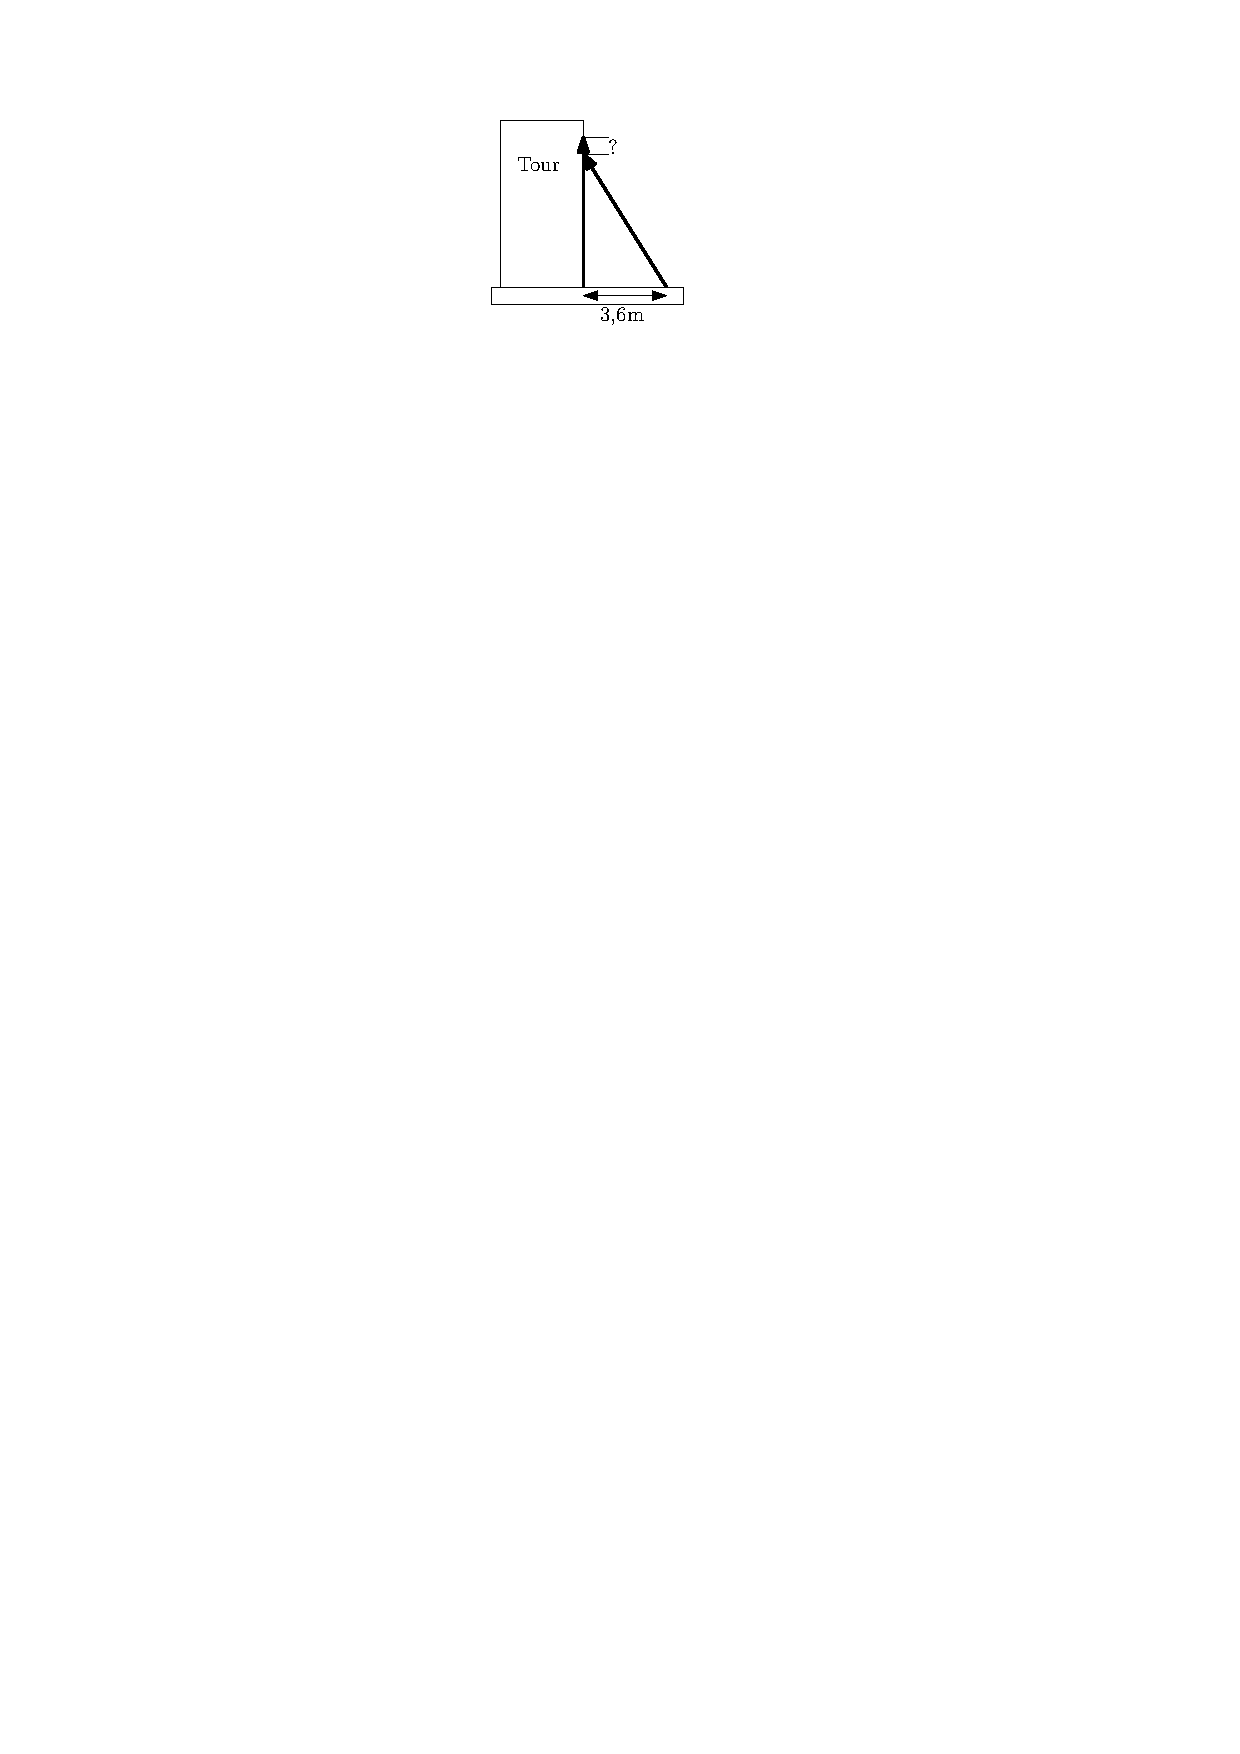
\includegraphics[width=0.6\linewidth]{4x6-Pythagore/pb3.pdf}
  \end{figure}
\end{enumerate}
\end{multicols}

\begin{enumerate}
  \item[pb4.] Fatma doit consolider et réparer un pont qui a été endommagé et qui risque de s'effondrer. Elle doit fixer 12 renforts en bois sur les poteaux verticaux qui soutiennent le ponton, comme le montre le dessin. \\
    \textbf{Calculer la longueur d'un renfort puis calculer la longueur totale de tous les renforts nécessaires}. 
  
    \begin{figure}[H]
    \centering
    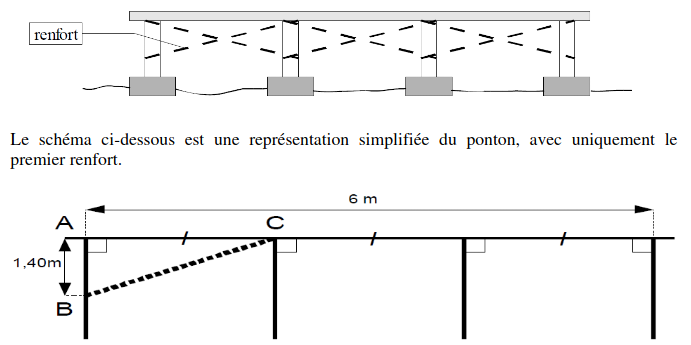
\includegraphics[width=0.8\linewidth]{4x6-Pythagore/pb4.png}
  \end{figure}
\end{enumerate}

\end{document}
